\documentclass[11pt]{l3deliverable}
\usepackage{geometry}
\usepackage{fullpage}
\usepackage{graphicx}
\usepackage{tabularx}
\usepackage{hyperref}
\usepackage{xcolor}
\definecolor{medium-red}{rgb}{0.35,0,0}
\hypersetup{colorlinks, linkcolor={medium-red}, citecolor={medium-red},
urlcolor={medium-red}}
\newcolumntype{T}{>{\centering\arraybackslash}m{0.20\textwidth}}
\newcolumntype{L}{>{\centering\arraybackslash}m{0.74\textwidth}}
\geometry{a4paper}
\setlength\parindent{0pt}
\title{System Design \& Acceptance Test Plan}
\deliverableID{D6}
\project{PSD3 Group Exercise 2}
\team{W}
\author{
    Gordon Reid: 1002536R\\
    Ryan Wells: 1002253W\\
    Kristopher Stewart: 1007175S\\
    David Selkirk: 1003646S\\
    James Gallagher: 0800899G\\
}
\date{\today}
\version{Final}
\begin{document}

\maketitle

\newpage

\tableofcontents

\newpage

\section{Introduction}

\subsection{Identification}

This is the design document and test plan for the internship management system
being developed by Team W for the Professional Software Engineering 3 course.
The internship management system is for Software Engineering (SE) and Electronic
and Software Engineering (ESE) students, studying in the school of Computing
Science.

\subsection{Related Documentation}

PSD3 Group Exercise Description:

\url{http://fims.moodle.gla.ac.uk/file.php/128/coursework/psd3-ge-2.pdf}

PSD3 Requirements Specification:

\url{fims.moodle.gla.ac.uk/file.php/128/coursework/requirements-specification-ge2.pdf}

\subsection{Purpose and Description Of Document}

This document serves as the design document containing the overall system
architecture diagram with associated state charts. Each component in the
system architecture also has its own class diagrams and API specifications
specified.

The latter section of the document contains the acceptance test plan for
the implementation of the Internship Management System.

\subsection{Document Status and Schedule}

This document is the draft version of the deliverable and is subject to major
change.

Change log:

\begin{enumerate}
\item Updated title page to be consistent with other deliverables.
\item Updated introduction section to include requirements specification document
link and states that the document contains the acceptance test plan.
\item Updated system architecture diagram based on feedback.
\end{enumerate}

\newpage

\section{System Architecture}

\subsection{Diagram}

\begin{centering}
  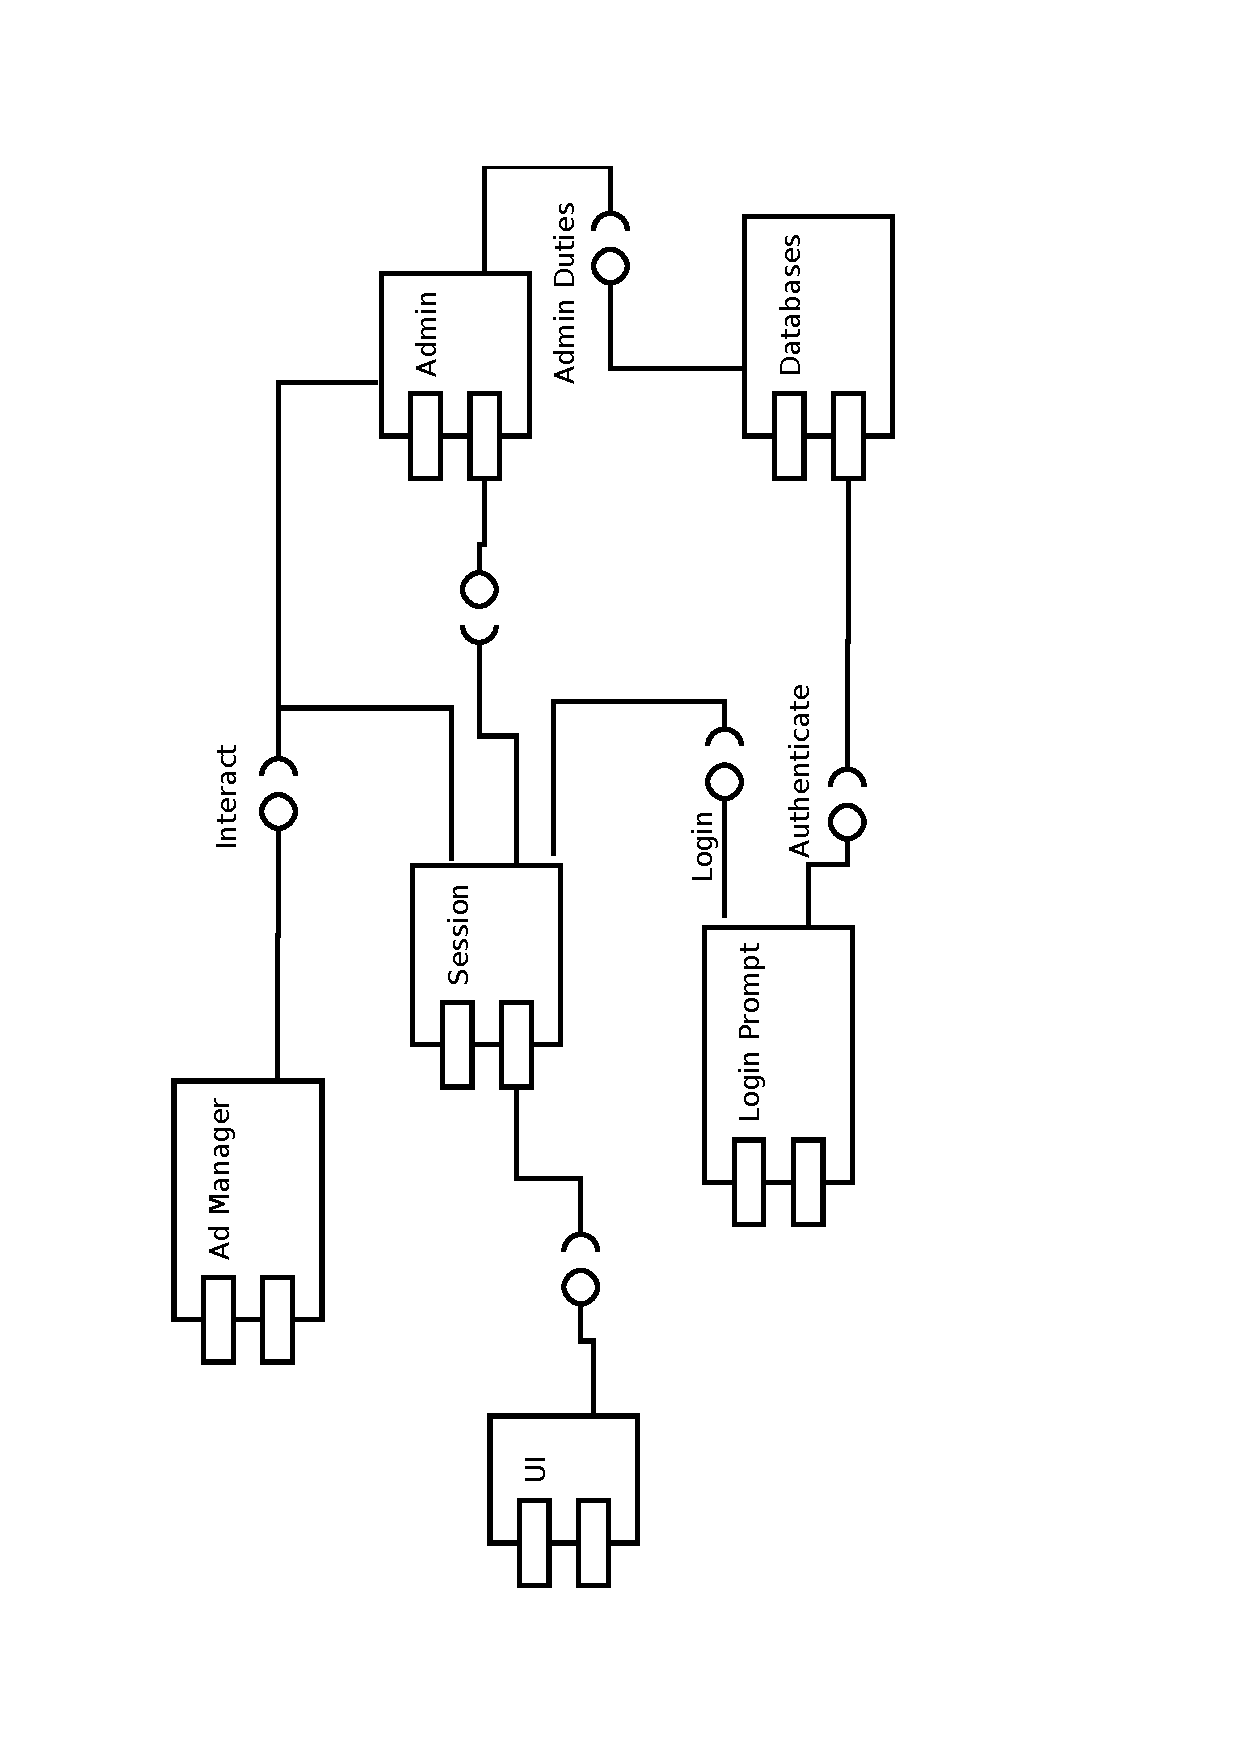
\includegraphics[width=\textwidth]{PSDDiagram.pdf}
\end{centering}

\subsection{Rationale}

We decided upon this system architecture as any component of the system should 
have the properties of being interchangeable with another substitutable 
component (substitutable defined as being having the same API). For this reason, 
we grouped related functionalities together and made them into a component. 
The `Ad Manager' and the `Databases' components could be combined together 
into one large `Database' component, but we did not want to create a coupling 
between these components - the `Ad Manager' may well have a database inside 
it, but the information inside this database is managed in a different way from 
the other data in the system such as users and companies.

All other components are defined by the primary reason that any component in the 
system can be replaced with no effect to the overall working of the system.

The `Session' component is essentially acting as a broker to user requests. This
simplifies the user interface's access to the functionality of the system and
further aids the ability for components to be swapped out with others as only
one component, the `Session' may have to be modified.

\newpage

\section{State Charts}

\subsection{Advertisement}

\subsubsection{Diagram}

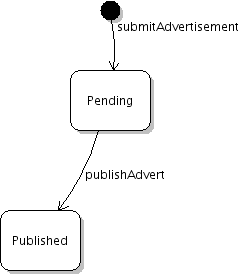
\includegraphics{advertState.png}

\subsubsection{Rationale}

The form of the state chart was decided based on the simplistic nature of an 
advertisements status. All adverts start off life as pending, after a company
has made the initial submission. They can be revised at any time prior to either
being declined by the course coordinator, where they are removed from the system
(and feedback sent to the company) or published for viewing.

An addition (which requires clarification) is the `Position Filled' state and
associated end state. This is asked in the questions section at the end of the
document. The question is number \ref{itm:advertDestroy}. As such, that part of 
the diagram is under review pending further information.

\subsection{Student}

\subsubsection{Diagram}

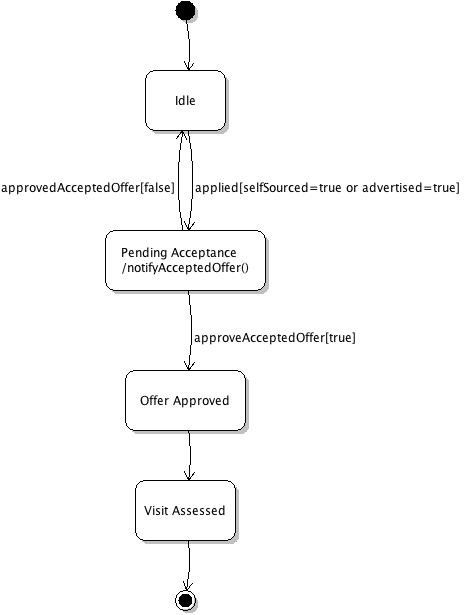
\includegraphics[width=0.9\textwidth]{studentState.png}

\subsubsection{Rationale}

We decided to create a state chart for a Student's flow through the
system as to clarify the functionality of the system with relation to
the student, and also for a base reason of a student having a
different state at multiple points in the system. There are various
paths that a student can take through this system and ultimately
result in the same final state, this is modelling the best case
scenario for a student where a student will eventually end up with an
approved final placement, which we have interpreted as being one of
the main functionalities of the system. 

A student continually changes state between `Idle' and `Pending
Acceptance' (through either `Applied for Position' or `Found Self
Sourced Role') potentially multiple times until a suitable position
has been found and only then they will progress on to `Offer
Approved'. A Student will then be stagnant until a visit has been
undertaken and then the student will terminate. A visit is outside the
control of the Student, so it will stay in this state until changed by
an outside element.

\newpage

\section{Class Diagrams and API Specifications}

\subsection{Advert Manager}

\subsubsection{Class Diagram}

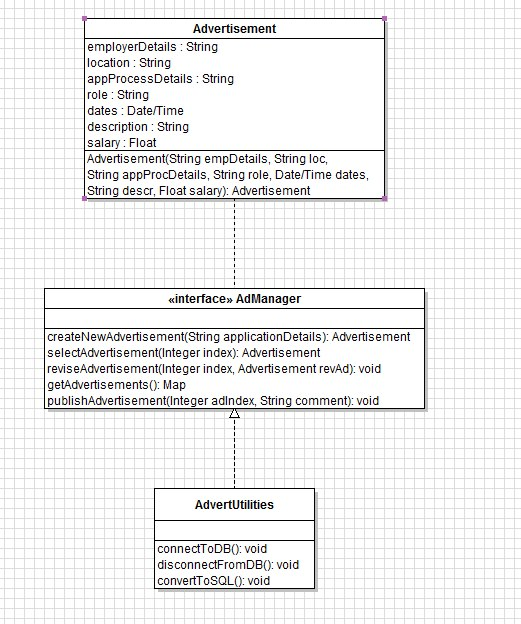
\includegraphics[width=\textwidth]{adManagerClassDiagram.png}

\subsubsection{API Specification}

\textbf{Full name}: public abstract interface AdManager\\

\textbf{Package}: uk.ac.glasgow.internman.AdManager

Each of the 3 available user types will be able to interact with this interface
but if the user has course coordinator rights then all available adverts can be
manipulated (published, denied etc), if they have registered employer rights
they'll be able to create/append and submit adverts for review and if they are
of type student, they'll only be able to view all published adverts.

\textbf{Methods}

\begin{itemize}

\item{\textbf{public Advertisement createNewAdvertisement(String applicationDetails)}

Create a new advert with the specified details

\textbf{Preconditions:} User must be of type Course Coordinator or Employer

\textbf{Postconditions:} Advert is created and appended to a list of adverts awaiting 
review within the database.}

\item{\textbf{public Advertisement selectAdvertisement(Integer index)}

Given an index, select and display the appropriate advert from the database.

\textbf{Preconditions:} Must be a valid index

\textbf{Postconditions:} Advert is displayed after the index was successfully matched
in the database.}

\item{\textbf{public void reviseAdvertisement(Integer index, Advertisement revise)}

Using an index to select an existing advert, change its contents with that of another supplied.

\textbf{Preconditions:} Must be a valid index

\textbf{Postconditions:} Advert is successfully replaced with the revised one and the changes
can be seen dependant on its state, by others.}

\item{\textbf{public Map getAdvertisements()}

For use mostly by students who wish to see all available published adverts.

\textbf{Preconditions:} Must be at least one published advert

\textbf{Postconditions:} Advert(s) are displayed one after another in the UI with their
descriptions displayed.}

\item{\textbf{public void publishAdvertisement(Integer adIndex, String comment)}

Course coordinator only, select an advert and give feedback to the employer on why the advert was published.

\textbf{Preconditions:} Must be a valid index, comment must be supplied.

\textbf{Postconditions:} State of the selected advert is changed to published and can be
successfully viewed by students.}

\end{itemize}
\newpage

\subsection{Session}

\subsubsection{Class Diagram}

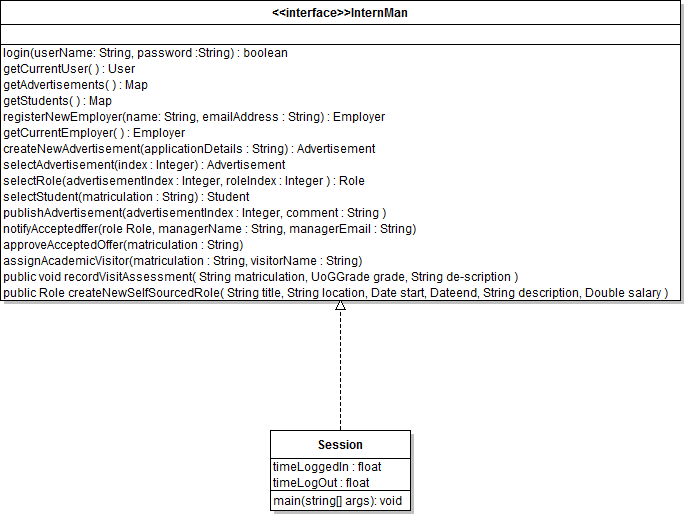
\includegraphics[scale=0.65,angle=90]{SessionClassDiagram.png}

\subsubsection{API Specification}

Session is purely the implementation of the supplied internship management
system API and doesn't supply functionality in its own right.

\newpage

\subsection{User Interface}

\subsubsection{Class Diagram}

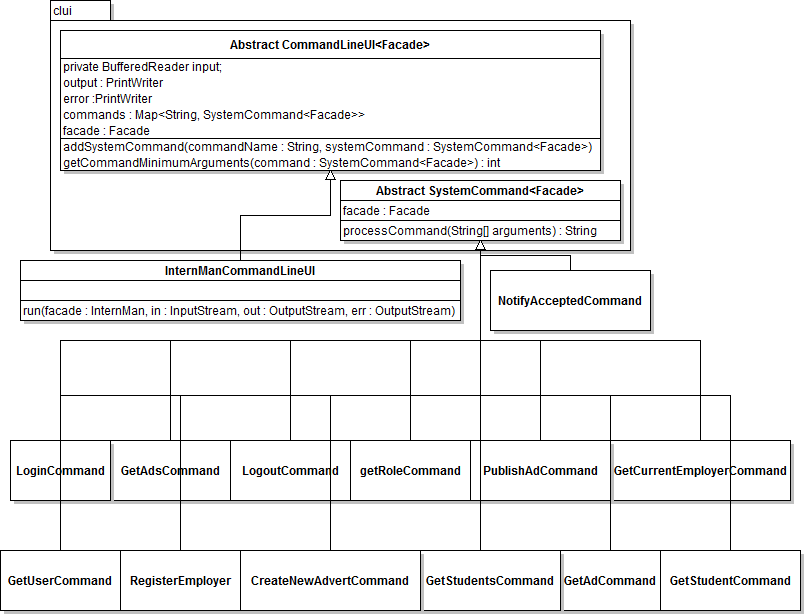
\includegraphics[scale=0.65,angle=90]{UIClassDiagram.png}

\subsubsection{API Specification}

\textbf{Full name:} public abstract interface InternManCommanLineUI\\

\textbf{Package:} uk.ac.glasgow.internman.ui\\

This is the interface for the graphical user interface.

\begin{itemize}

\item{\textbf{public void run(Facade facade, InputStream in, OutputStream out,
			OutputStream err)}

Runs the UI.

\textbf{Preconditions:} Facade must be constructed.

\textbf{Invariants:}

\textbf{Postconditions:} UI is displayed.}

\end{itemize}

\newpage

\subsection{Admin}

\subsubsection{Class Diagram}
\begin{centering}
  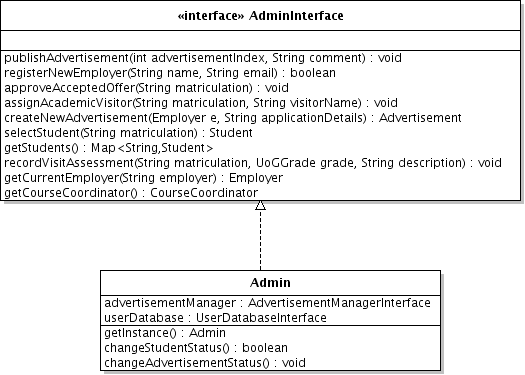
\includegraphics[width=0.7\textwidth]{adminClassDiagram.png}
\end{centering}
\subsubsection{API Specification}

\textbf{Full name:} public abstract interface Admin\\

\textbf{Package:} uk.ac.glasgow.internman.admin

This is the interface for the administration part of the database, accessible by
only the course coordinator.
This assumes that the user using this interface has Course Coordinator
rights.

\begin{itemize}

\item{\textbf{public void publishAdvertisement(Integer
    advertisementIndex, String comment)}

Approves an advertisement and makes it visible to students. Sends
comment as feedback to the employer as an email.

\textbf{Preconditions:} Advertisement must be in advertisement database.

\textbf{Invariants:}

\textbf{Postconditions:} Advertisement is now approved.}
%%%%%%%%%%%%%%%
\item{\textbf{public boolean registerNewEmployer(String name, String email)} 

Interface to add a company to the database, functionality is delegated to the
database component.
Error checking is done inside this function, but not whether or not a company
currently exists inside the companies database.

\textbf{Preconditions:} 

\textbf{Invariants:}

\textbf{Postconditions:} The return value of the delegated function indicates
the success of this function.}
%%%%%%%%%%%%%%%
\item{\textbf{public void approveAcceptedOffer(String matriculation)}

Approves the offer most recently accepted by the student with this matriculation
id. 
\textbf{Preconditions:} Student with this matriculation must have a successful
application and must have notified the Course Coordinator of their success.

\textbf{Invariants:} Student must not accept another successful application
during this review process.

\textbf{Postconditions:} Students status is changed to a success status.}
%%%%%%%%%%%%%%%
\item{\textbf{public void assignAcademicVisitor(String matriculation, String
    visitorName)}
Sends email to student, visitor and employer manager to let them know about
assignment. 

\textbf{Preconditions: An academic visit cannot be currently assigned.}

\textbf{Invariants:} 

\textbf{Postconditions:} }
%%%%%%%%%%%%%%%
\item{\textbf{public Advertisement createNewAdvertisement(String
    applicationDetails)}
Adds a new (not-yet-approved) advertisement into the system.

\textbf{Preconditions: Advertisement should not all ready exist in the
  system.}

\textbf{Invariants:} 

\textbf{Postconditions:} }
%%%%%%%%%%%%%%%
\item{\textbf{public Student selectStudent(String matriculation)}
Gets handle on Student from supplied matriculation.

\textbf{Preconditions: Null returned if Student is not in the map.}

\textbf{Invariants:} 

\textbf{Postconditions:} }
%%%%%%%%%%%%%%%
\item{\textbf{public void recordVisitAssessment( String matriculation,
    UoGGrade grade, String description)}
Records grade for visit. EMail to student and employer.

\textbf{Preconditions: A visit assessment should not currently be
  assigned for this student}

\textbf{Invariants:} 

\textbf{Postconditions:} }

\end{itemize}

\subsection{Login Prompt}

\subsubsection{Class Diagram}

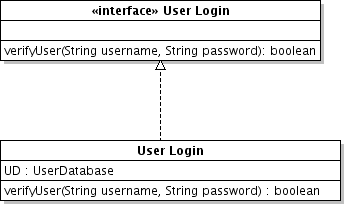
\includegraphics{loginClassDiagram.png}

\subsubsection{API Specification}

\textbf{Full name}: public abstract interface Login\\

\textbf{Package}: uk.ac.glasgow.internman.login

A user is presented with a prompt into which they must enter their MyCampus 
username and password. If the combination is valid, the user is logged in and 
presented with the summary of advertisements view.\\

\textbf{Methods}

\begin{itemize}

\item{\textbf{public Boolean verifyUser(String Id,String password)}

Check if a user is in database 

\textbf{Preconditions:} No user is currently logged in at the same user 
interface.

\textbf{Postconditions:} User is logged in, if username and password combination 
is correct.}

\item{\textbf{public Boolean userLoggedIn(String id)}

Check if a user is already logged in at the same user interface.}

\end{itemize}

\newpage

\subsection{Database}

\subsubsection{Class Diagram}

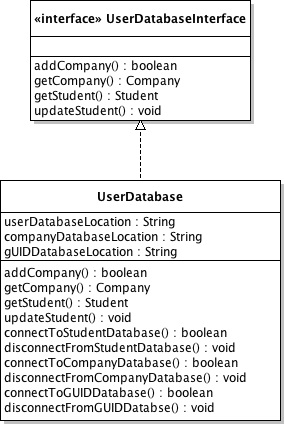
\includegraphics{databaseClassDiagram.png}

\subsubsection{API Specification}

\textbf{Full name:} public abstract interface UserDatabase\\

\textbf{Package:} uk.ac.glasgow.internman.users

This is the interface for the user database. This database will hold information
on students, companies, and the course coordinator. For University students and
staff members, the database will access the MyCampus GUID system for login. For
companies, a separate store for their user information will be used.\\

\textbf{Methods}

\begin{itemize}

\item{\textbf{public boolean addCompany(String name, String email, String 
password)}

Add information about a company to the database.

\textbf{Preconditions:} Database must not already contain details of the 
company.

\textbf{Invariants:}

\textbf{Postconditions:} Database now contains information about a company 
including their login password.}

\item{\textbf{public Company getCompany(String name)}

Gets information about the company with the given name.

\textbf{Preconditions:}

\textbf{Invariants:}

\textbf{Postconditions:} If a valid name is given, the object associated with
the company is returned, otherwise null is returned.}

\item{\textbf{public Student getStudent(String guid)}

Gets information about the student with the given GUID from MyCampus and the
application's user specific information database (such as internship progress).

\textbf{Preconditions:}

\textbf{Invariants:}

\textbf{Postconditions:} If a valid GUID is given, the object associated with
the student is returned, otherwise null is returned. If this is the first time
a student has been asked for, a record will be added to the user specific
information database.}

\item{\textbf{public void updateStudent(Student student)}

Updates the user specific data for the supplied student. For example, when a
student obtains an internship, or has had their internship assessed.

\textbf{Preconditions:} Student must be a valid Computing Science student and
is known to the application's user database.

\textbf{Invariants:}

\textbf{Postconditions:} Student's user specific information is up to date.}

\end{itemize}

\newpage

\section{Acceptance Test Plan}

\begin{tabularx}{\textwidth}{|T|L|}
\hline
Identifier & UtilityTCLogin1\\
\hline
Use Case & Login\\
\hline
Setup &\\
\hline
Interface & uk/ac/glasgow/internman\\
\hline
Includes &\\
\hline
Procedure & JUnit Test Case: uk/ac/glasgow/internman/tests/accept/LoginStudent\\
\hline
Inputs & String username: `9876543A', String password: `LetMeIn'\\
\hline
Outcome & Student with GUID `9876543A' is set as the current user of the system.
\\
\hline
\end{tabularx}

\vspace{2em}

\begin{tabularx}{\textwidth}{|T|L|}
\hline
Identifier & UtilityTCLogin2\\
\hline
Use Case & Login\\
\hline
Setup &\\
\hline
Interface & uk/ac/glasgow/internman\\
\hline
Includes &\\
\hline
Procedure & JUnit Test Case: uk/ac/glasgow/internman/tests/accept/LoginCompany\\
\hline
Inputs & String username: `TestCompany', String password: `LetMeIn'\\
\hline
Outcome & Company name `TestCompany' is set as the current user of the system.\\
\hline
\end{tabularx}

\vspace{2em}

\begin{tabularx}{\textwidth}{|T|L|}
\hline
Identifier & UtilityTCLogin3\\
\hline
Use Case & Login\\
\hline
Setup &\\
\hline
Interface & uk/ac/glasgow/internman\\
\hline
Includes &\\
\hline
Procedure & JUnit Test Case: uk/ac/glasgow/internman/tests/accept/LoginCC\\
\hline
Inputs & String username: `CourseCoordinator', String password: `LetMeIn'\\
\hline
Outcome & The course coordinator `CourseCoordinator' is set as the current user 
of the system.\\
\hline
\end{tabularx}

\vspace{2em}

\begin{tabularx}{\textwidth}{|T|L|}
\hline
Identifier & UtilityTCLogout1\\
\hline
Use Case & Logout\\
\hline
Setup & Some user is logged in.\\
\hline
Interface & uk/ac/glasgow/internman\\
\hline
Includes &\\
\hline
Procedure & JUnit Test Case: uk/ac/glasgow/internman/tests/accept/LogoutUser\\
\hline
Inputs &\\
\hline
Outcome & The current user is logged out and the corresponding session is
closed.\\
\hline
\end{tabularx}

\vspace{2em}
\begin{tabularx}{\textwidth}{|T|L|}
\hline
Identifier & ViewStudentSummary\\
\hline
Use Case & View student summary\\
\hline
Setup & User is logged in as Course Coordinator\\
\hline
Interface & uk/ac/glasgow/internman\\
\hline
Includes &\\
\hline
Procedure & JUnit Test Case: uk/ac/glasgow/internman/tests/accept/ViewStudentSummary\\
\hline
Inputs &\\
\hline
Outcome & Information about all students enrolled on the SESP course in the current session should be displayed\\
\hline
\end{tabularx}

\vspace{2em}

\begin{tabularx}{\textwidth}{|T|L|}
\hline
Identifier & UtilityAdSummary1\\
\hline
Use Case & View advertisement summary\\
\hline
Setup & user is logged in as Employer\\
\hline
Interface & uk/ac/glasgow/internman\\
\hline
Includes &\\
\hline
Procedure & JUnit Test Case: uk/ac/glasgow/internman/tests/accept/ViewAdSummaryEmployer\\
\hline
Inputs &\\
\hline
Outcome & Adverts belonging to TestCompany are returned\\
\hline
\end{tabularx}

\vspace{2em}

\begin{tabularx}{\textwidth}{|T|L|}
\hline
Identifier & UtilityAdSummary2\\
\hline
Use Case & View advertisement summary\\
\hline
Setup & user is logged in as Course Coordinator\\
\hline
Interface & uk/ac/glasgow/internman\\
\hline
Includes &\\
\hline
Procedure & JUnit Test Case: uk/ac/glasgow/internman/tests/accept/ViewAdSummaryCC\\
\hline
Inputs &\\
\hline
Outcome & All adverts, including unpublished ones, are returned\\
\hline
\end{tabularx}

\vspace{2em}

\vspace{2em}
\begin{tabularx}{\textwidth}{|T|L|}
\hline
Identifier & AdminTCRegisterEmployer\\
\hline
Use Case & Register Employer\\
\hline
Setup & \\
\hline
Interface & uk/ac/glasgow/internman\\
\hline
Includes & UtilityTCLogin3\\
\hline
Procedure & JUnit Test Case: uk/ac/glasgow/internman/tests/accept/RegEmpl\\
\hline
Inputs & String name: ``MegaCorp'', String email ``bossman@megacorp.com''\\
\hline
Outcome & Company ``MegaCorp'' is added as a user to the system with
the above details.\\
\hline
\end{tabularx}

\vspace{2em}

\begin{tabularx}{\textwidth}{|T|L|}
\hline
Identifier & AdminTCApproveOffer\\
\hline
Use Case & Approve Accepted Offer\\
\hline
Setup & Must be one advertisement relating to the submitted details.\\
\hline
Interface & uk/ac/glasgow/internman\\
\hline
Includes & UtilityTCLogin3\\
\hline
Procedure & JUnit Test Case: uk/ac/glasgow/internman/tests/accept/Approve\\
\hline
Inputs & String matriculation: ``0024601J''\\
\hline
Outcome & The most recent accepted placement for the above
matriculation is accepted.\\
\hline
\end{tabularx}

\vspace{2em}

\begin{tabularx}{\textwidth}{|T|L|}
\hline
Identifier & AdManTC1\\
\hline
Use Case & View Advertisement Detail\\
\hline
Setup &\\
\hline
Interface & uk/ac/glasgow/internman/AdManager\\
\hline
Includes &\\
\hline
Procedure & JUnit Test Case: uk/ac/glasgow/internman/tests/accept/ViewAd\\
\hline
Inputs & Integer index: 44\\
\hline
Outcome & If supplied index is valid, the advert will be displayed on screen
\\
\hline
\end{tabularx}

\vspace{2em}

\begin{tabularx}{\textwidth}{|T|L|}
\hline
Identifier & AdManTC2\\
\hline
Use Case & Submit Advertisement\\
\hline
Setup &\\
\hline
Interface & uk/ac/glasgow/internman/AdManager\\
\hline
Includes &\\
\hline
Procedure & JUnit Test Case: uk/ac/glasgow/internman/tests/accept/SubAd\\
\hline
Inputs & String applicationDetails: `me incorporated | spain | stuff | programmer | 10/06/2013-10/10/2013 | description | 10000`\\
\hline
Outcome & Advert is created and appended to database with this information linked to it
\\
\hline
\end{tabularx}

\vspace{2em}

\begin{tabularx}{\textwidth}{|T|L|}
\hline
Identifier & AdManTC3\\
\hline
Use Case & Revise Advertisement\\
\hline
Setup &\\
\hline
Interface & uk/ac/glasgow/internman/AdManager\\
\hline
Includes &\\
\hline
Procedure & JUnit Test Case: uk/ac/glasgow/internman/tests/accept/RevAd\\
\hline
Inputs & Integer index: 24, Advertisement revised\\
\hline
Outcome & Advert is matched in database to index and it's details are switched with the supplied advert.
\\
\hline
\end{tabularx}

\vspace{2em}

\begin{tabularx}{\textwidth}{|T|L|}
\hline
Identifier & AdminTCPublishAdvertisement\\
\hline
Use Case & Publish Advertisement\\
\hline
Setup & Must be one advertisement relating to the submitted details.\\
\hline
Interface & uk/ac/glasgow/internman\\
\hline
Includes & UtilityTCLogin3\\
\hline
Procedure & JUnit Test Case: uk/ac/glasgow/internman/tests/accept/Publish\\
\hline
Inputs & Integer advertisementIndex: ``24601'', String comment:
``I hope this helps you find the man you are looking for!''\\
\hline
Outcome & The advertisement with the above index is now published for
a student to view and the comment is sent to the company that
published the advertisement.\\
\hline
\end{tabularx}

\vspace{2em}

\begin{tabularx}{\textwidth}{|T|L|}
\hline
Identifier & StudentTCNotifiyAccepted\\
\hline
Use Case & Publish Notify accepted offer\\
\hline
Setup & Role below must exist in the system.\\
\hline
Interface & uk/ac/glasgow/internman\\
\hline
Includes & UtilityTCLogin1\\
\hline
Procedure & JUnit Test Case: uk/ac/glasgow/internman/tests/accept/Notify\\
\hline
Inputs & Role role: ``Software Engineer'', String managerName: ``Chris
P. Bacon'', String managerEmail: ``manager@company.com'')\\
\hline
Outcome & The student who has invoked this function has sent an email
to the course coordinator about this placement success.\\
\hline
\end{tabularx}

\vspace{2em}

\begin{tabularx}{\textwidth}{|T|L|}
\hline
Identifier & TCAssignVisitor\\
\hline
Use Case & Assign Academic Visitor\\
\hline
Setup & A student has an approved placement and is ready to have their
placement visit.\\
\hline
Interface & uk/ac/glasgow/internman\\
\hline
Includes & UtilityTCLogin1\\
\hline
Procedure & JUnit Test Case: uk/ac/glasgow/internman/tests/accept/AssignVisitor\\
\hline
Inputs & Student name who has internship, Visitor name and email.\\
\hline
Outcome & The Visitor is notified which student they are to visit. The student's
record is updated with the visitor information.\\
\hline
\end{tabularx}

\begin{tabularx}{\textwidth}{|T|L|}
\hline
Identifier & TCRecordVisit\\
\hline
Use Case & Record Visit Assessment\\
\hline
Setup & A student has a visit assigned that has just been completed. The 
assigned grade needs to be added to the student's record.\\
\hline
Interface & uk/ac/glasgow/internman\\
\hline
Includes & UtilityTCLogin1\\
\hline
Procedure & JUnit Test Case: uk/ac/glasgow/internman/tests/accept/RecordVisit\\
\hline
Inputs & Student name who has internship, description of student's
performance, and associated grade..\\
\hline
Outcome & The student's record has a grade and textual description regarding
their performance during the internship.\\
\hline
\end{tabularx}


\newpage

\section{Requirements Specification Questions}

\begin{enumerate}

\item{Employers are required to register however during the registration process
only the company name and email is supplied (registerNewEmployer()). However,
users are required to supply their username and password to login. Based on the
assumption that the employer/company name is the username, what would the
password initially be set to?}

\item{How does the course coordinator decline an offer a student has received?}

\item{\label{itm:advertDestroy} When and how does an approved/published 
advertisement disappear from the set of available advertisements?}

\end{enumerate}

\end{document}
